% Metaphor: pipeline. One direction, one stage after another, nothing
% doubling back -- reach for it when the thing being drawn is a sequence
% and the reader's question is "what happens next".
%
% Idiom: a chain placed with `positioning`. Each stage says where it sits
% relative to the one before it, so inserting a stage moves everything
% downstream instead of re-opening every adjacency by hand.
% House palette (docs/TIKZ-STYLE.md). These five lines travel *inside*
% every figure that uses them -- not a shared file, not a preamble: the
% renderer injects only \usepackage{tikz}, and a thesis fragment is
% \input into a document that has never heard of this project.
\definecolor{cgInk}{HTML}{1A1A1A}
\definecolor{cgFlow}{HTML}{0072B2}
\definecolor{cgAccent}{HTML}{D55E00}
\definecolor{cgAlt}{HTML}{009E73}
\definecolor{cgAux}{HTML}{56B4E9}
\usetikzlibrary{positioning}
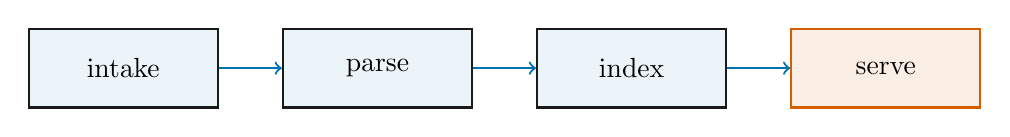
\begin{tikzpicture}[thick,
                    stage/.style={draw=cgInk,align=center,fill=cgFlow!8,
                                  minimum width=24mm,minimum height=10mm}]
  \node[stage] (intake) {intake};
  \node[stage,right=8mm of intake] (parse) {parse};
  \node[stage,right=8mm of parse] (index) {index};
  % The one accented node: `cgAccent` marks what the figure is about.
  \node[stage,right=8mm of index,draw=cgAccent,fill=cgAccent!10] (serve) {serve};
  \draw[->,cgFlow] (intake) -- (parse);
  \draw[->,cgFlow] (parse) -- (index);
  \draw[->,cgFlow] (index) -- (serve);
\end{tikzpicture}
